\section{Further Work}

A significant problem concerning the optimization via ZX-Calculus, which is actively being researched, is the development of efficient extraction algorithms. Such algorithms are needed because when we are done simplifying a circuit, we are left with a compact ZX-Diagram. Since we want to be able to simulate the optimized circuit, we need to specify an algorithm that extracts a classical circuit out of ZX-Diagrams. This generally is not a trivial task since ZX-Diagrams are a superset of the classical quantum circuits\cite{duncan2020simplification} as seen in figure \ref{fig:extraction}, which means that not every ZX-Diagram corresponds to a valid quantum circuit. An important optimization procedure is keeping enough information about the quantum circuit to allow for an extraction of a classical circuit after the simplification. \cite{duncan2020simplification}.

\begin{figure}[h]
    \centering
    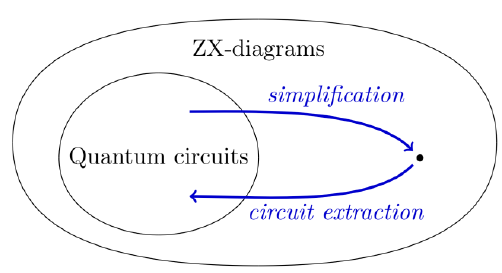
\includegraphics[width=0.35\textwidth]{images/extraction.png}
    \caption{Simplifcation process\cite{duncan2020simplification}}
    \label{fig:extraction}
\end{figure}